%نام و نام خانوادگی:
%شماره دانشجویی: 
\مسئله{}
 یکی از دامنه‌های کاربرد نرم‌افزار \lr{Software Product Line} یا خط تولید نرم‌افزار است.\\
الف) منظور از خط تولید نرم‌افزار چیست؟ به طور کامل و همراه با مثال آن را بررسی نمایید. \\
ب) چه مزایایی دارد؟ حداقل 5 مورد بیان شود.

\پاسخ{

الف)  گاهی شرکت‌ها و سازمان‌ها به دنبال تولید نرم‌افزارهایی هستند که از یک خانواده‌ی مشترک هستند و عملکردی مشابه دارند. در این‌صورت تولید جداگانه‌ی هرکدام از نرم‌افزارها به‌صرفه نیست و از مفهوم خط نرم‌افزار تولید (SPL) استفاده می‌شود. خط تولید نرم‌افزار به مجموعه‌ای از سیستم‌های مبتنی بر نرم‌افزار (software-intensive) گفته می‌شود که شامل ویژگی‌های مدیریت‌شده‌ و عمومی مشترکی هستند که نیازهای یک بخش خاص از بازار یا یک ماموریت را برآورده می‌کنند. این ویژگی‌ها براساس مجموعه‌ی مشترکی از دارایی‌ها اصلی ( \Ir{assets core} ) به‌صورت تجویزی توسعه‌ داده‌شده‌اند (به این معنی که روش تولیدشان جداگانه و یا سلیقه‌ای نیست). بعد از برقرار شدن خط توليد نرم‌افزار، دارایی‌های قابل استفاده مجدد در مخزن دارايی‌های اصلی ذخيره می‌شوند و برای محصولات دارایی‌های مناسب تشخیص داده می‌شوند و تنظیمات لازم روی آن‌ها صورت می‌گیرد تا در کنار سایر دارایی‌ها قرار گرفته و از تجمیع‌شان محصول تولید شود.

مثال: فرض کنید شرکت تولید لوازم دیجیتالی وجود دارد که برای محصولاتش از سیستم‌عامل‌های مختلفی استفاده می‌کند.

\begin{figure}[h]
	\centering
	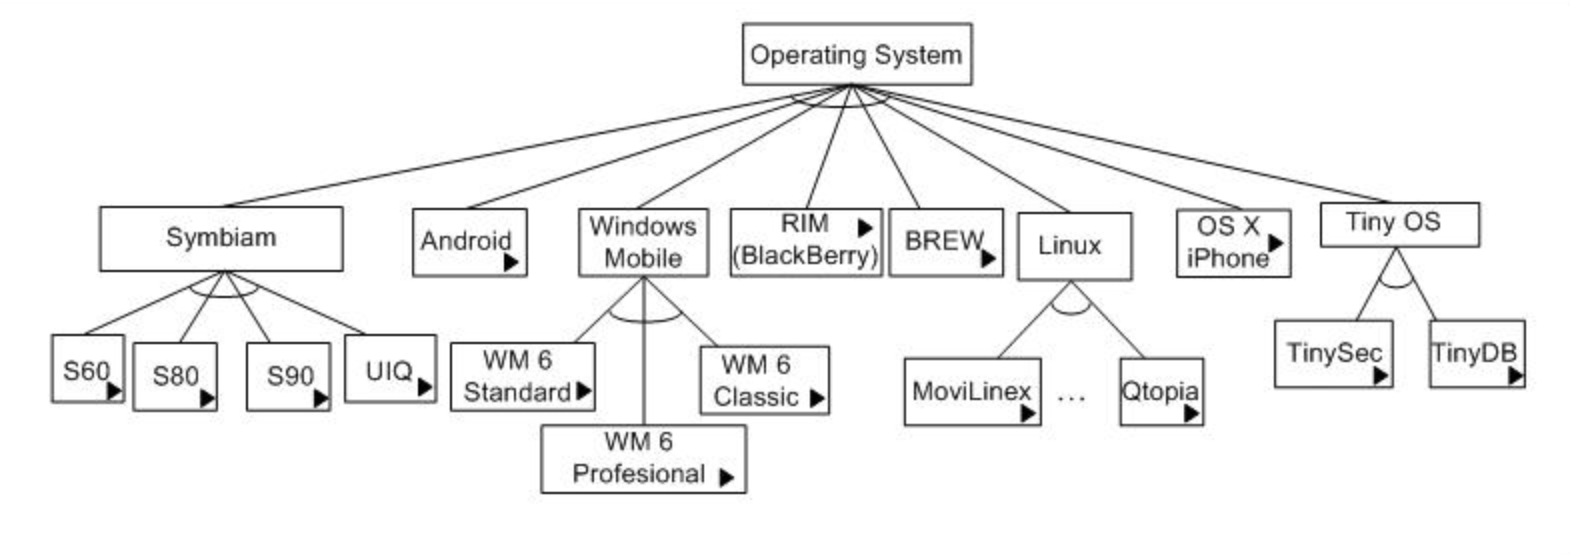
\includegraphics[scale=0.55]{figs/1-3}
	\caption{سیستم‌عامل‌های محصولات}
\end{figure}

درواقع اینجا نوع سیستم‌عامل یکی از ویژگی‌هایی است که می‌توان بر اساس آن بین محصولات دسته‌بندی انجام داد و  خط‌های تولید را به‌راه انداخت. یعنی برای تولید محصولاتی که دارای سیستم‌عامل اندروید هستند، مسیری متفاوت از مسیر تولید محصولات دارای سیستم‌عامل OS را طی می‌کنند و غیره. حال خود این سیستم‌عامل‌ها هم از طریق assetهایی که از قبل مشخص شده‌اند (مانند تست‌کیس‌ها، مستندات و نیازمندی‌ها) توسعه داده‌می‌شوند که این assetها در مخزنی ذخیره می‌شوند. البته این تنها از دید سیستم‌عامل بود و برای سخت‌افزار و دیگر بخش‌های محصولات هم می‌توان دسته‌بندی انجام داد و خط‌ تولید ایجاد کرد.

ب)فواید استفاده از SPL در ادامه آورده‌شده‌اند:
\begin{enumerate}

\item 
بهبود کیفیت محصول: در تولید یک خط نرم‌افزار، به ابعاد مختلف توجه می‌شود و تست‌های بسیاری انجام می‌شوند تا از عملکرد خط تولید اطمینان پیدا کنند. بنابراین محصولات در طول ساخت‌شان بارها مورد آزمایش قرار می‌گیرند و نیز پس از ساخت‌ بازبینی می‌شوند تا اشکالات‌شان برطرف شوند.
\item 
مدیریت پیچیدگی: با استفاده‌ مجدد از دارایی‌ها، پیچیدگی تولید محصولات کمتر می‌شود.
\item
مدیریت تکامل: دارایی‌های اصلی را می‌توان در محصولات مختلف پیاده‌سازی کرد و به این صورت آن‌ها را تکامل داد. در این‌صورت سازماندهی تکامل نیز آسان‌تر و بهتر خواهد بود.
\item 
کاهش هزینه‌های توسعه: در ابتدا برای ایجاد یک خط تولید سرمایه‌ی زیادی نیاز است اما با گذر زمان نسبت به تولید جداگانه‌ی محصولات کم‌خرج‌تر خواهد بود چراکه هربار محصولات از صفر تولید نمی‌شوند و نیاز نیست برای بعضی بخش‌ها هزینه‌ کرد.
\begin{figure}[h]
	\centering
	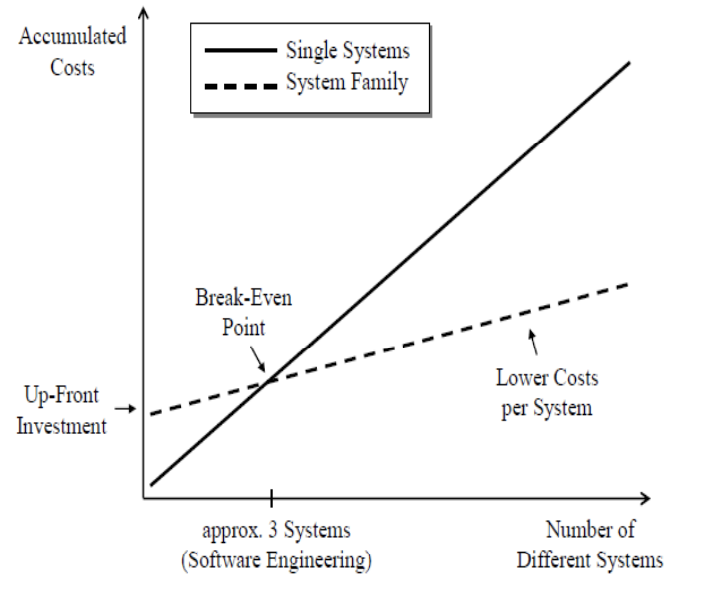
\includegraphics[scale=0.55]{figs/1-1}
	\caption{نمودار هزینه‌ بر حسب تعداد سیستم‌ها}
\end{figure}

\item 
کاهش زمان عرضه به بازار  ( \Ir{market to time} ):
در اوایل SPL نیاز به زمان زیادی دارد تا مجموعه دارایی‌ها را استخراج کند (که نسبت به تولید انفرادی محصولات زمان بیشتری می‌گیرد) اما بعد از مدتی و با استفاده‌ی مجدد از دارایی‌ها، زمان عرضه کاهش می‌یابد چراکه دیگر محصولات از صفر ساخته نمی‌شوند.

\begin{figure}[h]
	\centering
	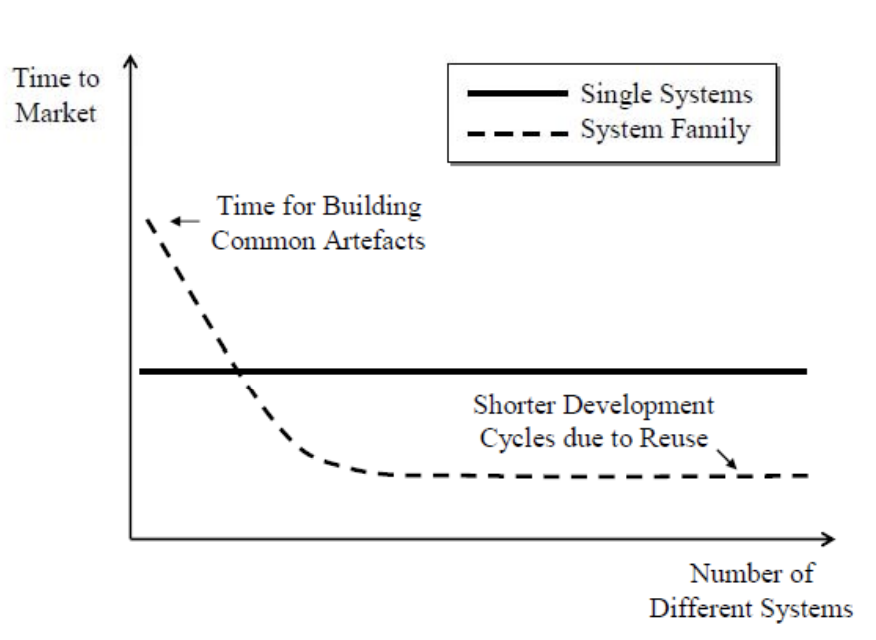
\includegraphics[scale=0.5]{figs/1-2}
	\caption{نمودار زمان عرضه به بازار‌ بر حسب تعداد سیستم‌ها}
\end{figure}

\item
استفاده موثرتر از منابع: در خط تولید، از دارایی‌ها و منابعی که موجود هستند مجددا استفاده می‌توان کرد و دور انداخته نمی‌شوند.
\item 
کاهش ریسک و خطرات تولید: با هربار تولید یک محصول از طریق خط تولید، اطمینان به کارکرد آن بیشتر می‌شود. همچنین هربار با آزمون‌هایی که انجام می‌شود، دقت خط تولید بالاتر می‌رود و درصورتیکه مشکلی وجود داشته باشد، برطرف می‌شود.
\item 
کاهش کمی نیروی انسانی: در استفاده از خط تولید، نیاز به ساخت بعضی از قسمت‌ها برای محصولات نیست و درنتیجه نیروی انسانی‌ کمتری نیاز خواهد بود.
\item 
پیکربندی و شخصی سازی سریع: می‌توان تمامی محصولات یک دسته را صرفا با تغییر دارایی‌ها، متناسب با نیازهای مشتری درآورد و شخصی‌سازی کرد. این شخصی‌سازی سرعت بالایی دارد چرا که محصولات از صفر پیاده‌سازی نمی‌شوند و تغییرات هم به‌صورت گروهی روی آن‌ها اعمال می‌شوند و نه تک‌تک.
\item
افزایش رضایت مشتری: مشتریان محصولات با کیفیت بالاتر را در مدت زمان کوتاه‌تری دریافت می‌کنند. همچنین به‌علت ظاهر مشابهی که محصولات دارند، مشتریان بعد از کار کردن با یکی از آن‌ها می‌توانند به راحتی با بقیه‌شان نیز کار کنند.
\item
بهبود تخمين هزينه‌ها: از آنجایی که برای تولید محصولات از دارایی‌های یکسانی استفاده می‌شود، محاسبه‌ی هزینه‌های تولید آسان‌تر و دقیق‌تر خواهد بود.

\end{enumerate}

\section*{مراجع:}

\begin{latin}
	\begingroup
	\renewcommand{\section}[2]{}%
	
\begin{thebibliography}{9}
%   https://www.student.unsw.edu.au/how-do-i-cite-electronic-sources

	\bibitem{item1}
	Carnegue Mellon University,
	\textit{SEI Digital Library},
	Software Product Lines Collection, 
	accessed 7 November 2022,
	\url{https://resources.sei.cmu.edu/library/asset-view.cfm?assetid=513819}
	
\end{thebibliography}
\endgroup
\end{latin}


% https://resources.sei.cmu.edu/library/asset-view.cfm?assetid=513819

% http://caosd.lcc.uma.es/wp-content/resources/spl/index.htm

% https://edisciplinas.usp.br/pluginfile.php/4109317/mod_resource/content/2/Aula6b-SPLE-Jaejoon.pdf

% http://facultymembers.sbu.ac.ir/s_khoshnevis/ASE951/ASE-Session04-SPL.pdf

% https://virgool.io/@rabbani\_mohammad/%D8%AE%D8%B7-%D8%AA%D9%88%D9%84%DB%8C%D8%AF-%D9%86%D8%B1%D9%85-%D8%A7%D9%81%D8%B2%D8%A7%D8%B1-xrtqyacpy0i6

}